% LaTeX Template for Project Report, Version 2.0
% (Abstracted from a Major Project Report at CSED, NIT Calicut but can be
% modified easily to use for other reports also.)
%
% Released under Creative Commons Attribution license (CC-BY)
% Info: http://creativecommons.org/licenses/by/3.0/
%
% Created by: Kartik Singhal
% BTech CSE Batch of 2009-13
% NIT Calicut
% Contact Info: kartiksinghal@gmail.com
%
% It is advisable to learn the basics of LaTeX before using this template.
% A good resource to start with is http://en.wikibooks.org/wiki/LaTeX/
%
% All template fields are marked with a pair of angular brackets e.g. <title here>
% except for the ones defining citation names in ref.tex.
%
% Empty space after chapter/section/subsection titles can be used to insert text.
%
% Just compile this file using pdflatex after making all required changes.

% This open source template is being utilized by me (Sameer Shaikh) to implement the
% Final Report for my final year B.E. project. The above text has been kept
% as an acknowledgement of the original author's work.

\documentclass[12pt,a4paper]{report}
\usepackage[pdftex]{graphicx} %for embedding images
\usepackage{url} %for proper url entries
\usepackage[bookmarks, colorlinks=false, pdfborder={0 0 0}, pdftitle={Machine Learning On Real-time Data To Enhance Home Automation}, pdfauthor={Sameer Shaikh}, pdfsubject={Machine Learning Application}, pdfkeywords={<keywords here>}]{hyperref} %for creating links in the pdf version and other additional pdf attributes, no effect on the printed document
%\usepackage[final]{pdfpages} %for embedding another pdf, remove if not required
\usepackage{verbatim} %defines comment environment
\usepackage{float} %for 'H' option in \begin{figure}[H]

\usepackage{fancyhdr} %for headers and footers
\pagestyle{fancy}
\lhead{}
\chead{Machine Learning To Enhance Home Automation}
\rhead{\thepage}
\lfoot{}
\cfoot{Department of Computer Engineering, AAEMF’s Pune}
\rfoot{}

\begin{document}
\renewcommand\bibname{References} %Renames "Bibliography" to "References" on ref page
%\renewcommand\bibname{} %Renames "Bibliography" to a blank on ref page
\renewcommand{\footrulewidth}{0.4pt} %default is 0pt; add horizontal line above footer

%include other pages
\begin{titlepage}

\begin{center}

\textup{\small A\\{\bf Preliminary Project Report}\\On}\\[0.2in]

% Title
\Large \textbf {``Machine Learning On Real-time Data To Enhance Home Automation"}\\[0.25in]

       \small \emph{Submitted to}
        \vspace{.1in}

       {\bf Savitribai Phule Pune University}\\[0.1in]
        
       \small \emph{FOR THE DEGREE\\
        OF}
        \vspace{.1in}

       {\bf Bachelor of Computer Engineering}\\[0.25in]

% Submitted by
\normalsize BY \\
\begin{table}[h]
\centering
\begin{tabular}{ll} \\
%Names of Students & Exam Seat Number\\
\\
\\
Mr. Ayyaj Attar & B120634202\\
Mr. Sameer Shaikh & B120634211\\ 
Mr. Siddik Pathan & B120634216\\ \\
\end{tabular}
\end{table}

\vspace{.1in}
Under the guidance of\\
{\textbf{Prof. R. Shaikh}}\\[0.2in]

\vfill

% Bottom of the page

\includegraphics[width=0.27\textwidth]{./InitialPages/al_ameen-logo}\\[0.1in]
\Large{Department of Computer Engineering}\\
\normalsize
\textsc{Al-Ameen College of Engineering}\\
Pune -- 412 216 \\
\vspace{0.2cm}
Year 2016-2017

\end{center}

\end{titlepage}

\newpage
\thispagestyle{empty}


\begin{center}

\begin{comment}
\huge{Department of Computer Engineering}\\[0.5cm]
\normalsize
\textsc{Al-Ameen College of Engineering Pune}\\[1.5cm]
\end{comment}

\begin{figure}
	\centering
	
\includegraphics[width=0.27\textwidth]{./InitialPages/al_ameen-logo}
\end{figure}

\emph{\LARGE Certificate}\\[2.0cm]
\end{center}
\paragraph{}
\normalsize This is to certify that,\\
\hspace*{3cm}\textbf{Mr. AYYAJ ATTAR} \hfill Exam Seat No: B120634202\\
\hspace*{3cm}\textbf{Mr. SAMEER SHAIKH} \hfill Exam Seat No: B120634211\\
\hspace*{3cm}\textbf{Mr. SIDDIK PATHAN} \hfill Exam Seat No: B120634216\\\\
\noindent
have  successfully completed their preliminary project report entitled \linebreak``\textbf{MACHINE \ LEARNING \ ON \ REAL--TIME \ DATA \ TO \ ENHANCE \ HOME \ AUTOMATION}", under our supervision and guidance in partial fulfillment of the requirements for the degree of Bachelor of Engineering in Department of Computer Engineering of Savitribai Phule Pune University during the academic year 2016-2017.
\\[1.0cm]

\begin{comment}
\begin{table}[h]
\centering
\begin{tabular}{ll}
Names of Students & Exam Seat Number\\ \\ \hline
\\
Mr. Ayyaj Attar & <Exam Seat Number> \\ 
Mr. Sameer Shaikh & <Exam Seat Number> \\
Mr. Siddik Pathan & <Exam Seat Number> \\
\end{tabular}
\end{table}
\end{comment}

\vfill
%\addvspace{6.0cm}

% Bottom of the page
%\hspace{-0.625cm}
\begin{center}
\parbox[t][][b]{0.5\textwidth}{\flushleft Prof. R. Shaikh\\\textbf{\hspace*{0.9cm}Guide}}\parbox[t][][b]{0.5\textwidth}{\flushright Prof. G. S. Kothawale\\\textbf{HOD\hspace*{1.6cm}}}\\[1.0cm] %Signs of Guide & HoD

\parbox[t][][b]{\textwidth}{\centering \textbf{Principal}\\\textbf{AAEMF's COE \& MS}}\\[1.0cm] %Principal's sign

\parbox[t][][b]{0.5\textwidth}{\flushleft \textbf{Internal Examiner}\\}\parbox[t][][b]{0.5\textwidth}{\flushright \textbf{External Examiner}}\\ %Sign of Internal guide & External Examiner
\end{center}

%\parbox[0.5\textwidth]{\centering (Head of Department)}
%\parbox[0.5\textwidth]{\centering (Project Guide)}

%following is the original bottom of the page
\begin{comment}

% Bottom of the page
\begin{flushright}
<Guide name here>\\
(Project Guide)\\[1.5cm]
<Coordinator name here>\\
(Course Coordinator)\\
\end{flushright}

\end{comment}

\begin{flushleft}
Date:\\
Place:
\end{flushleft}

\newpage
\thispagestyle{empty}

\begin{center}

PROJECT APPROVAL SHEET\\[3\baselineskip]



{\small A Project Report Titled as}\\[\baselineskip]

\textbf{{\large Machine Learning on Real-time Data to Enhance Home Automation}}\\[\baselineskip]

Is verified for its originality in documentation, problem statement, proposed\\
work and implementation successfully completed by\\[2\baselineskip]


\textbf{Mr. AYYAJ ATTAR} Exam Seat No: B120634202\\
\textbf{Mr. SAMEER SHAIKH} Exam Seat No: B120634211\\
\textbf{Mr. SIDDIK PATHAN} Exam Seat No: B120634216\\[\baselineskip]

at\\[4\baselineskip]




DEPARTMENT OF COMPUTER ENGINEERING\\
\textbf{AAEMF’S}\\
\textbf{College of engineering and management studies,}\\
\textbf{Koregaon Bhima}\\
SAVITRIBAI PHULE PUNE UNIVERSITY, PUNE\\
ACADEMIC YEAR 2016-2017\\

\vfill

\noindent
\hspace*{0.75cm}Prof. R. Shaikh \hfill Prof. G. S. Kothawale\hspace*{0.25cm} \\
\hspace*{1.75cm}Guide \hfill H.O.D.\hspace*{1.5cm} \\
Dept. of Computer Engg. \hfill Dept. of Computer Engg.


\end{center}
%\cleardoublepage
%\pagebreak
%\phantomsection
%\addcontentsline{toc}{chapter}{Acknowledgements}
\chapter*{Acknowledgments}
\thispagestyle{empty}
%\vspace{1.0in}
\paragraph{}
It is a great pleasure for us to acknowledge the assistance and contribution of a number of individuals and entities who helped us in presenting this project report on \textbf{``Machine Learning On Real-time Data To Enhance Home Automation"}.
\paragraph{}
First and foremost we wish to record our gratitude and thanks to - our Project Guide \textbf{Prof. Rukaiya Shaikh}, the Head of Department \textbf{Prof. G.S. Kothawale}, and the \textbf{Principal, Mrs. S. Kapse} - for their guidance, instruction and enthusiasm leading to the successful completion of this report.
\paragraph{}
This acknowledgement would be incomplete without expressing our special thanks to the authors and organizations maintaining the various open-source tools that we have used in our work - especially to Linus Torvalds for his college project that turned into what we know today as the Linux Kernel.
\paragraph{}
Last but not the least, we would like to thank our parents, friends and our colleagues who helped us directly or indirectly in successfully completing this project report.
\\
\begin{flushright}
\parbox[t][][l]{0.3\textwidth}{\textbf{Mr. Ayyaj Attar\\Mr. Sameer Shaikh\\Mr. Siddik Pathan\\}}\\
(B.E. Computer Engg.)
\end{flushright}

\vfill

\begin{center}
AAEMF’s, Department of Computer Engineering, 2016-17
\end{center}
%Date:\\%ORIGINAL
%Place:\\%ORIGINAL
\newpage

\vspace{2in}

\begin{comment}

\newpage
\begin{center}
\begin{Huge}
\textbf{Abstract}
\end{Huge}
\end{center}

\end{comment}

\begin{abstract}

\paragraph{}
Traditional home automation systems are mostly hard-coded or require manual automation plan generation by users. This requires interaction between a control system (an interface) and the user, requiring quite some effort and time to be put in manual planning of the home environment. This project intends to explore applying ML on real-time usage data to generate personalized and time-variant home automation plans. These plans will save the user time and effort, leading to a smoother ML driven home automation experience. We collect streaming usage statistics from smart-home occupants and store it on a centralized server. Simultaneously, we also collect “external” data (which may consist of environmental factors like natural light intensity, wind speed, et cetera) which may influence occupants’ usage behavior. These datasets are combined, with data timestamps as a unique identifying field, into a super-set. It’s then fed into a Machine Learning system to correlate user habits with time of the day and the external factors. The correlation hence established will be updated in real time. This correlation will be in the form of a prediction model that will be used to predict near future values of target devices for the occupant. Hence, by combining real-time usage data from a conventional home automation system and Machine Learning, we will be able to provide smoother and more comfortable environment to the users, as the burden of plan generation will be greatly reduced.

\end{abstract} 


\pagenumbering{roman} %numbering before main content starts
\tableofcontents
\listoffigures
\listoftables
%\listofabbreviations % To be included.

\newpage
\pagenumbering{arabic} %reset numbering to normal for the main content

%\chapter{Problem Definition}

<Problem Definition here>
 %objective changed to problem definition %Currently not relevant
\chapter{Introduction}

%%%%%%%%%%%%%%%%
\begin{comment}

\section{Background and Recent Research}
\subsection{<any sub section here>}

\subsection{Literature Survey}

\subsubsection{<Sub-subsection title>}
some text\cite{citation-1-name-here}, some more text

\subsubsection{<Sub-subsection title>}
even more text\footnote{<footnote here>}, and even more.

\section{Motivation}

\end{comment}
%%%%%%%%%%%%%%%%

\section{Detailed Problem Definition}
\paragraph{}
Most present-day smart homes use simple reflex agents for automation. Simple reflex agents are non-flexible and can work with limited percepts and hard-coded actuation rules. These rules may not suit all people. This rigidity in usability of present consumer automation systems forms the core of our problem.
\paragraph{}
We intend to develop a software solution to this problem, that is centered around machine learning. This solution will be in the form of a learning agent that learns user habits by observation and anomaly detection.

\section{Brief Description}
\paragraph{}
This project aims to enhance the home automation experience by collecting usage data from the user and applying prediction algorithms on it to predict the next step the user may take. Furthermore, external data will also be collected an correlated with the usage data in order to determine what external conditions may influence the user's behavior. This involves data like weather data and traffic data.

%\section{Problem Definition}

	% Overview
	% Breif Description
	% Problem Definition
\chapter{Analysis}

% Project Plan
% Requirement Analysis
% Team Structure

\section{Project Plan}
\begin{figure}[h]
	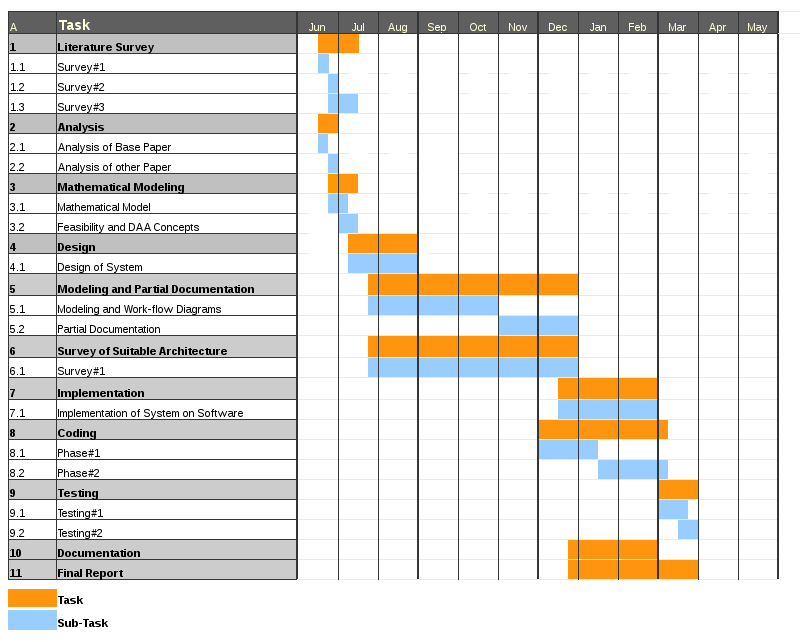
\includegraphics[width=\textwidth]{./Chapter2/gantt-chart}
		\caption{Project Plan}
\end{figure}

\section{Requirement Analysis}
\paragraph{}
<Content>

\section{Team Structure}
\paragraph{}
<Content> %previously, literature-survey.tex
	% Project Plan [TO BE ADDED]
	% Requirement Analysis [TO BE ADDED]
	% Team Structure [TO BE ADDED]
\chapter{Design}

% Software Requirements
% Hardware Requirements
% Software Requirements Specification
	% Functionality
		% What is the software supposed to do?
	% External Interface
		% How does the software interact with people, the system's hardware, other hardware, and other software?
		% What assumptions can be made about these external entities?
	% Required Performance
		% What is the speed, availability, response time, recovery time of various software functions and so on?
	% Quality Attributes
		% What are the portability, correctness, maintainability, security, and other considerations?
	% Design Constraints imposed on an implementation
		% Are there any required standards in effect, implementation language, policies for database integrity, resource limits, operating environment(s) and so on?

\section{Software Requirements}
\paragraph{}
For the PC (LaaS server):
\begin{enumerate}
\item Any operating system with a Python interpreter available
\item Python 2.7
\item Flask micro-framework for implementing web service (package ``flask")
\item SciKit Learn ML library for Python (package ``sklearn")
\end{enumerate}

\paragraph{}
For the Raspberry Pi (device controller):
\begin{enumerate}
\item Raspbian OS for the Pi
\item Python 2.7
\item Flask micro-framework for implementing controller's web interface (package ``flask")
\end{enumerate}

\section{Hardware Requirements}

\begin{enumerate}
\item A personal computer
\item A Raspberry Pi Single Board Computer (SBC)
\item Proper network infrastructure
\end{enumerate}

\pagebreak

\section{Software Requirements Specification}

\subsection{Functionality}
\paragraph{}
We intend the software to be divided over two tiers: the interface and the LaaS Server. The user is served up a web interface to the smart devices connected to the Raspberry Pi over a conventional TCP/IP network. It will be possible to view the states of individual devices and change them. Such usage of the system can happen even in the absence of the Machine Learning Service. That is to say, the first tier consists of an independent interfacing system that enables the user to control connected smart devices, and this may optionally utilize a usage-prediction-oriented machine learning service if it is available.
\paragraph{}
The second tier consists of a special case of SaaS (Software-as-a-Service), called LaaS (Learning-as-a-Service). This service is intended to provide proper WebAPI for the tier one application to communicate with. Data can be sent by the tier one application to the LaaS service using this API, which will then be processed continuously to generate predictions for individual devices. These predictions can also be requested by the tier one application so it can apply it in real-time to the smart environment it is providing an interface to. Non-availability of the services in this tier will not affect the user interfacing system implemented in the first tier, except for the unavailability of predictions.
\paragraph{}
Unavailability of the first tier, id est interface tier, is fatally deteriorating to the user experience. This tier must always be available and smoothly working, that is to say, it should be robust. The second tier provides a service which is not necessarily central to  the functioning of the smart home by design. This means that unavailability of the service will not affect the core control system provided by the first tier.

\pagebreak
\subsection{External Interfaces}
\paragraph{}
Interfacing between different components of this system is crucial to it's execution. We will use conventional communication mechanisms like RESTful WebAPIs for communication between both the client \& first tier, and the first \& second tier.
\begin{figure}[H]
		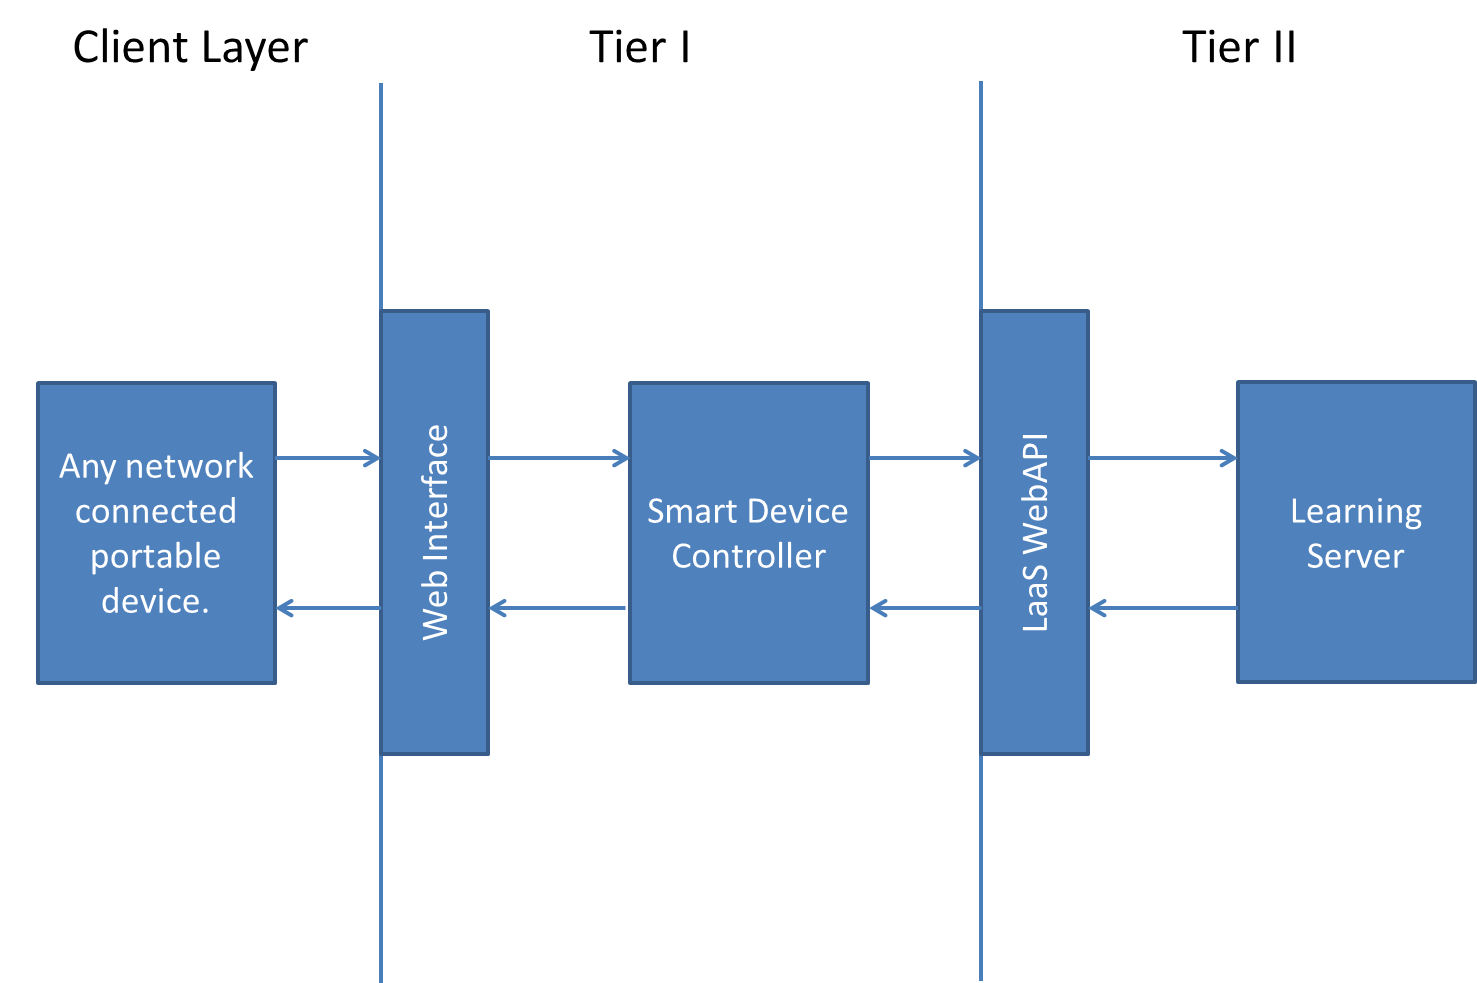
\includegraphics[width=\textwidth]{./Chapter3/client-t1-t2}
			\caption{Overview of Tiered Components and their Interfacing}
	\end{figure}
	\subsubsection*{Client - Tier I Interface}
	\paragraph{}
	The smart environment can be controlled via a web app. This app can be accessed by the user by connecting to the smart devices' controller (the Raspberry Pi) on the standard HTTP Port (port 80). The user can then view current states of the connected smart devices and change them according to their preference.
	\begin{figure}[H]
		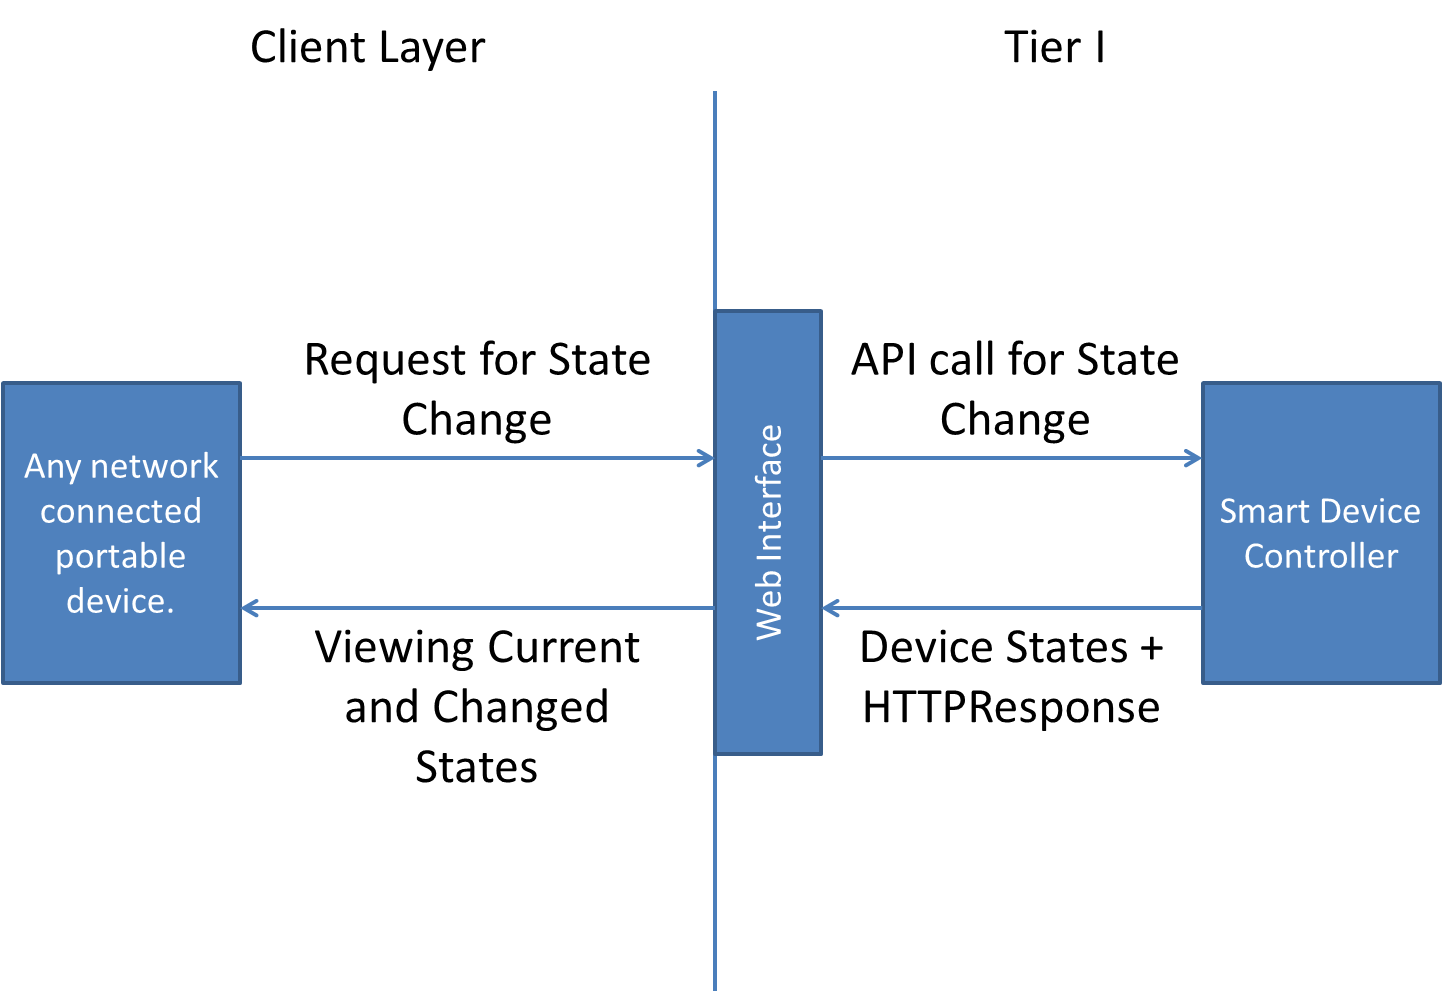
\includegraphics[width=\textwidth]{./Chapter3/client-t1}
			\caption{Interface between Client and Tier I}
	\end{figure}
	\paragraph{}
	Besides collecting user generated actions, the controller may also collect external data (like current weather) in order to facilitate prediction of user actions based on regressive correlation with external influncers.
	\paragraph{}
	This interface is critical as it delivers the frontend for our system to the user. Network delay or inconsistencies within its implementation directly and drastically affect user experience.
	
	\subsubsection*{Tier I - Tier II Interface}
	\paragraph{}
	The LaaS server can be accessed by the Tier I application through a RESTful WebAPI. The API includes calls for collecting device state changes made by the user and for requesting the prediction based on recent usage data.
	\begin{figure}[H]
		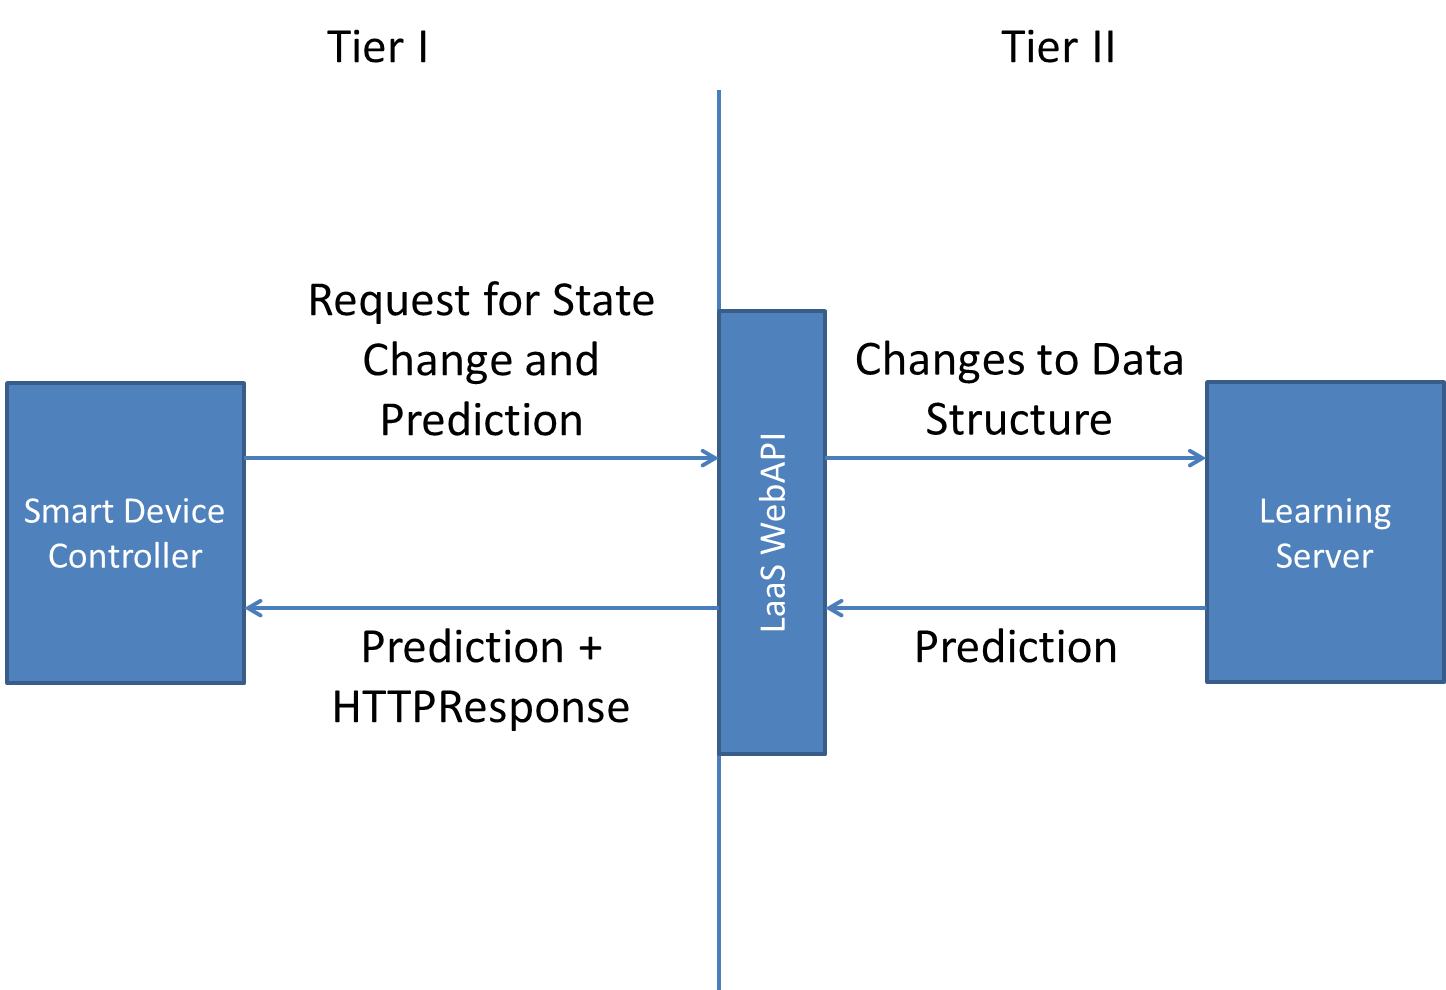
\includegraphics[width=\textwidth]{./Chapter3/t1-t2}
			\caption{Interface between Tier I and Tier II}
	\end{figure}
	\paragraph{}
	The only job of the LaaS server is to learn correlations between user actions and external influencing factors, and report the predictions thus generated back to the controller upon request. This server may be hosted locally within the controller's LAN, or publicly, as an on-cloud SaaS Service.

\pagebreak
\subsection{Required Performance}
\paragraph{}
The performance of this system completely depends on the performance of individual machines and the speed their communication. This requires us to again describe the required performance with respect to individual tiers.
\subsubsection*{Tier I}
\paragraph{}
This tier is performance critical and must always be available to the user. This is mainly because it serves the interface to the smart home environment, which is the most basic functional requirement of our system.
\paragraph{}
Besides, this tier should be able to work even with the unavailability of Tier II, which provides a supplementary, non-essential service. Also, the delay between the client and Tier I interface should be unnoticeable, as it can directly impact user experience as well as usability.

\subsubsection*{Tier II}
\paragraph{}
This tier is not as critical to the performance of the system as Tier I. Although unavailability of the services provided by this system can deteriorate the user experience and usability, it will not render the system totally unusable, unlike Tier I.
\paragraph{}
While the system is running, it is expected to serve up predictions based on current actions quick enough that the user doesn't notice the delay. To achieve this, we need to make sure that the machine that hosts this server is fast enough to achieve this, and also that the network delay between the two tiers is the minimum possible.

\pagebreak
\subsection{Quality Attributes}
\paragraph{}
This section describes the attributes that determine the quality of the software being written. The three attributes that we can identify within this system are Availability, Usability, and Functionality.
\subsubsection*{Availability}
\paragraph{}
The system should provide at least a minimal device control interface at all times. Although, it should also provide proper and timely predictions for the user's actions most of the time. Then we can say that this system has an acceptable record of availability.

\subsubsection*{Usability}
\paragraph{}
The system should be easy to handle for the user and provide a simple interface. Delay between an interface action (pressing a button) and response (changes in device states) should be minimal to the point of being unnoticeable. This requires the interfaces between client \& Tier I, and Tier I \& Tier II to be implemented with the main focus on speed. Such an implementation can be achieved using Responsive UI Design paradigms.

\subsubsection*{Functionality}
\paragraph{}
Functionality of the system can be judged based on whether the right components and services are provided and work the way they're expected to. This involves observing how well the system responds to user actions and in what ways. Also, the responses generated should be in line with the developed tests. Each test case should be satisfied by the system at least under ideal condition, like availability of services and network connectivity.

\paragraph{}
Functionality of any system is subject to its usage, environment, et cetera, just as well as it is to its implementation. Nonetheless, we try to include as many possible test cases as are practically possible during the time of development.

\pagebreak
\subsection{Design Constraints}
\paragraph{}
This system is entirely designed using Python (for the back-end on Tier I and II) and HTML/Javascript (for the front-end on Tier I). Tier I is implemented on a Raspberry Pi 2, model B+ - an ARM Cortex A7-based 32-bit quad-core Single Board Computer with 512 MB RAM and frequency of 900 MHz, and running the default Raspbian OS. Python is installed by default on these systems. With this, we need to install the python-flask package - a lightweight framework for implementing robust WSGI applications.
\paragraph{}
Tier II is targeted  towards conventional PCs, and should execute smoothly on mid-level to performance-level PCs as well as workstations and servers. For our implementation, we've used a Linux distribution with Python 2, python-flask (Flask web framework library) and python-sklearn (SciKit Learn ML library) installed. Other operating systems that have a Python interpreter available for them can also be used.
\paragraph{}
The system can be initiated by running the following individual modules:
\begin{enumerate}
\item Raspberry Pi module, which implements the user interface to the smart devices and the connection and control logic for the connected devices. This module forms the Tier I of the system.
\item Server module, which can run on a conventional personal computer and implements the "brains" of the system. That is to say, it provides the system with usage-learning capabilities in the form of a conventional WebAPI. This module forms the Tier II of the system.
\end{enumerate}
\paragraph{}
For communication, we use conventional TCP/IP network. This implementation is currently targeted towards LAN-based in-home usage and purposefully leaves out even common security features in order to manifest the core idea in a simple way.
	% Rename to "Design" [DONE]
	% Software Requirement
	% Hardware Requirement
	% SRS [DONE]
\chapter{Modelling}

% Data Flow Diagram
% State Transition Diagram

\section{Data Flow Diagram}

\begin{figure}[h]
	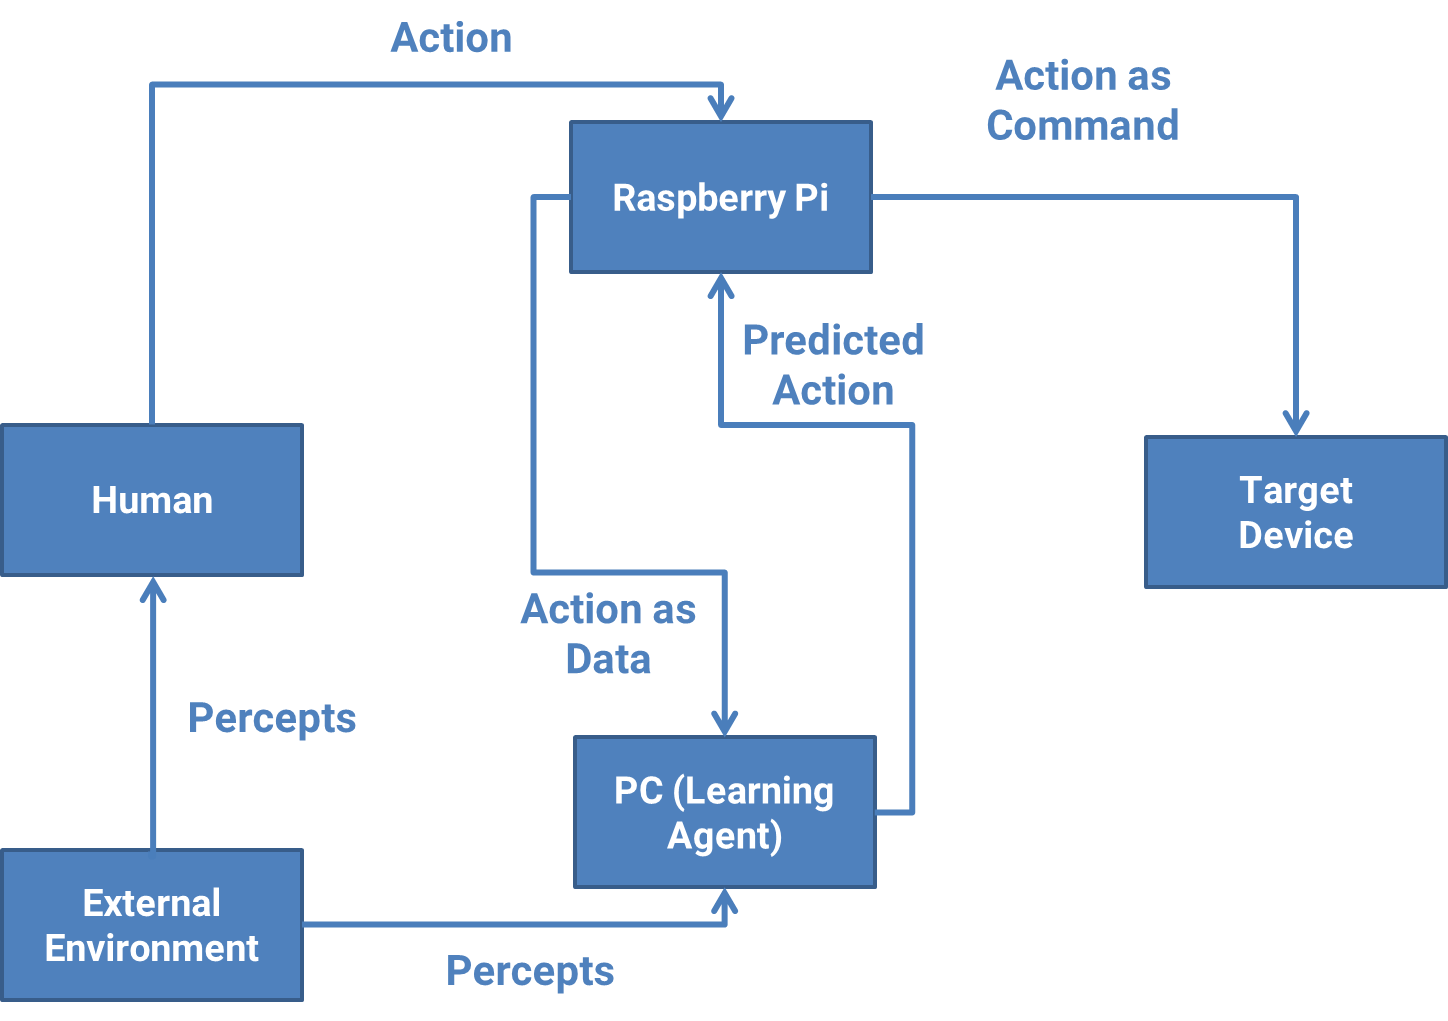
\includegraphics[width=\textwidth]{./Chapter4/dfd}
		\caption{Data Flow Diagram}
\end{figure}

\section{State Transition Diagram}

\begin{figure}[h]
	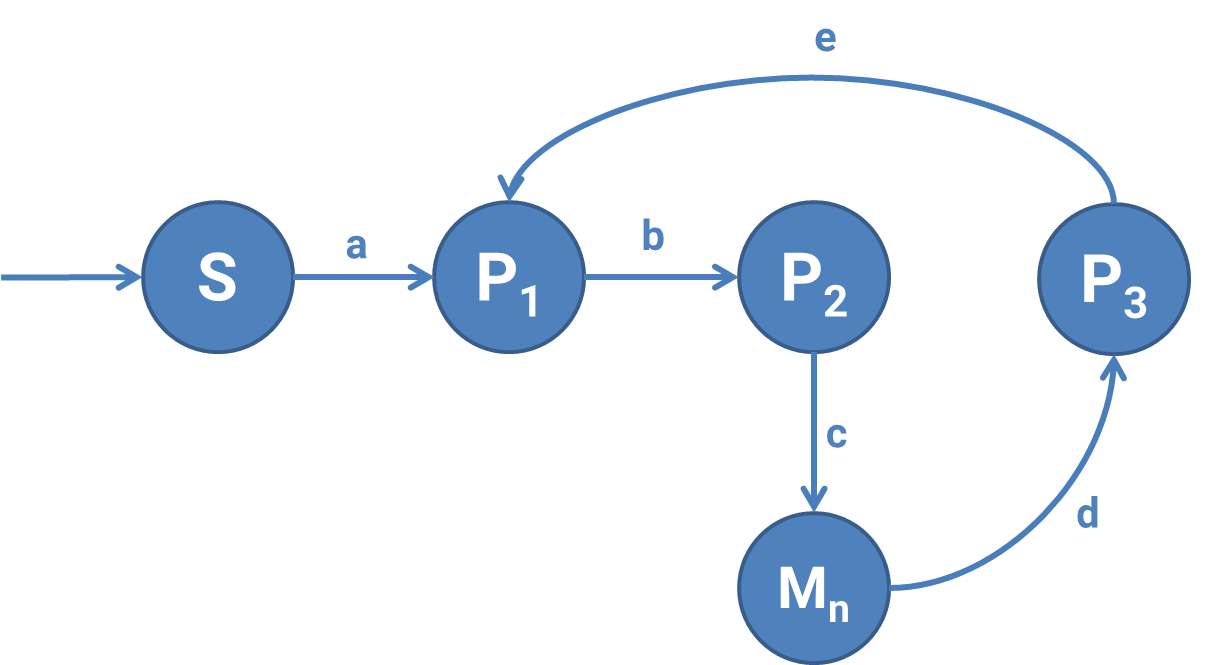
\includegraphics[width=\textwidth]{./Chapter4/state-transition}
		\caption{State Transition Diagram}
\end{figure}

Where,\\
\hspace*{1cm} S: Start state\\
\hspace*{1cm}P1: Phase 1- Observation and collection of usage data.\\
\hspace*{1cm}P2: Phase 2- Run machine learning algorithms on collected data to generate a prediction model.\\
\hspace*{1cm}Mn: Prediction Model- Current (nth) prediction model. n is the total number of discrete anomalies detected since start.\\
\hspace*{1cm}P3: Phase 3- Detect anomalies and modify data collected in Phase 1 to match the anomalies.\\\\
\hspace*{1cm}a: Create a mutable table for holding observed data for the learning agent to process.\\
\hspace*{1cm}b: Data collection threshold reached or data modification completed.\\
\hspace*{1cm}c: Prediction Model generated.\\
\hspace*{1cm}d: Anomaly detected. This implies change in user habit or detection of a new habit.\\
\hspace*{1cm}e: Make corrections in the table to avoid anomalies in the near future.\\

\paragraph{}
Our system does not have any state of absolute success. Success and failure are both temporary and the system is designed to learn from its mis-predictions. The canonical success in this project will be the usability of the machine learning system. The more data it is exposed to, the more successful the prediction model will be.

\begin{comment}
\begin{figure}
	\includegraphics[width=\textwidth]{Flower}
		\caption{A Flower}
\end{figure}
\end{comment}
	% Rename to "Modelling" [DONE]
	% Data Flow Diagram
	% State Transition Diagram
\chapter{System Design}

% System Architecture
% UML Diagrams
	% Use Case Diagram
	% Class Diagram
	% Activity Diagram
	% Sequence Diagram

\section{System Architecture}

	\begin{figure}[h]
		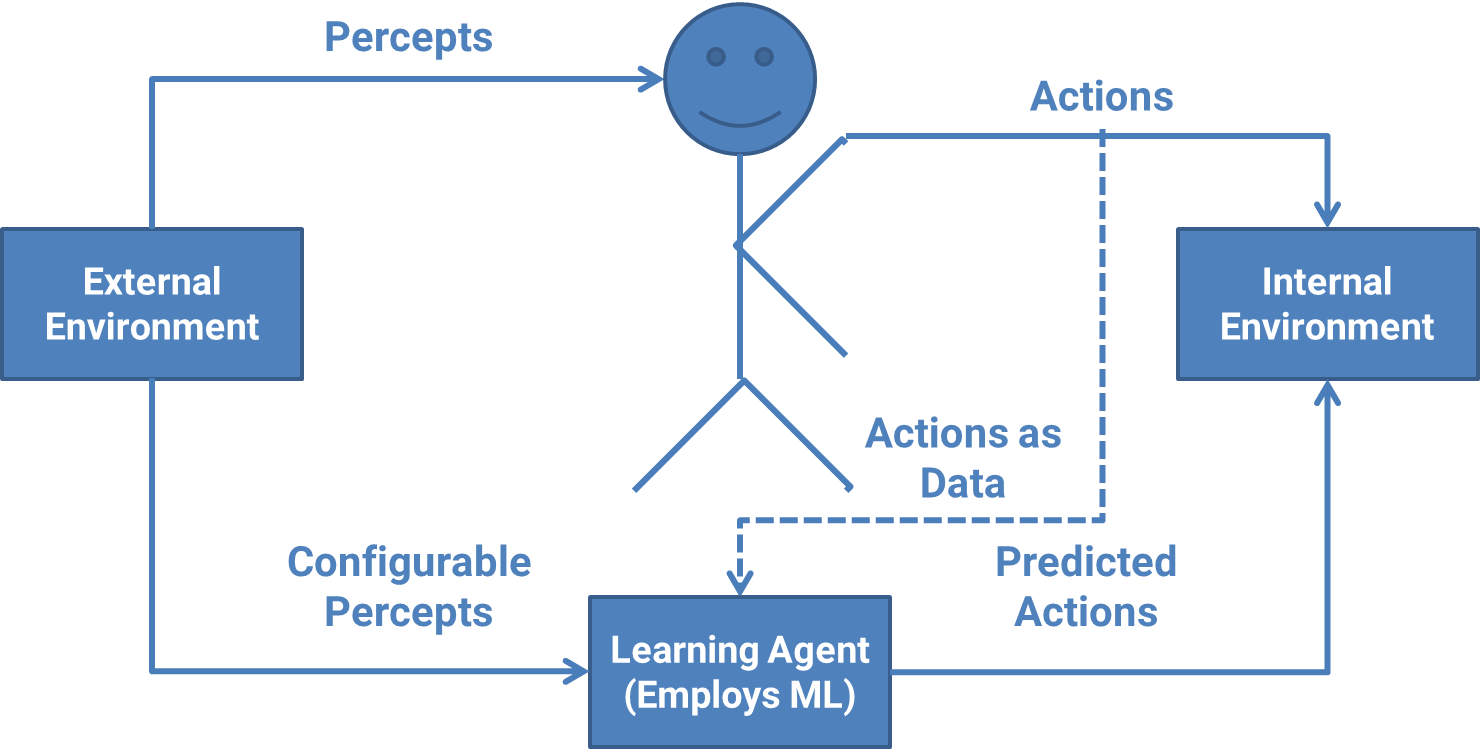
\includegraphics[width=\textwidth]{./Chapter5/system-architecture}
			\caption{System Architecture}
	\end{figure}
	\paragraph{}
	This defines the major elements within our system, their arrangement and interaction. It essentially represents an agent-environment model with the human and the Learning Agent as the two agents.

\section{UML Diagrams}

	\subsection{Use Case Diagram}
	\begin{figure}[H]
	\centering
	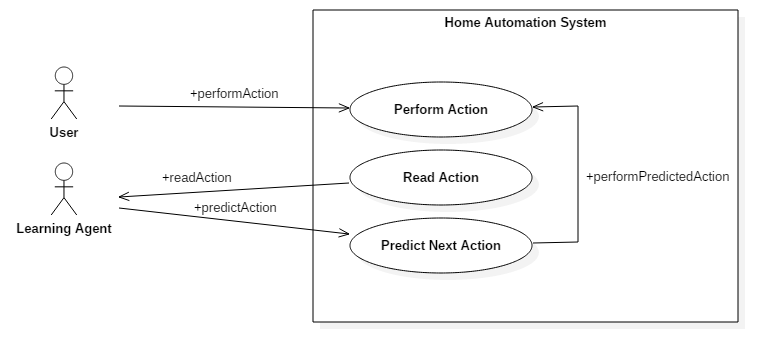
\includegraphics[width=\textwidth]{./Chapter5/UseCaseDiagram}
		\caption{Use Case Diagram}
	\end{figure}
	\paragraph{}
	This represents the various use cases that are possible in our system. The human user is the primary actor which may perform certain actions to initiate learning in a secondary learning agent that mimics the user's usage patterns.
	
	\subsection{Class Diagram}
	\begin{figure}[H]
	\centering
	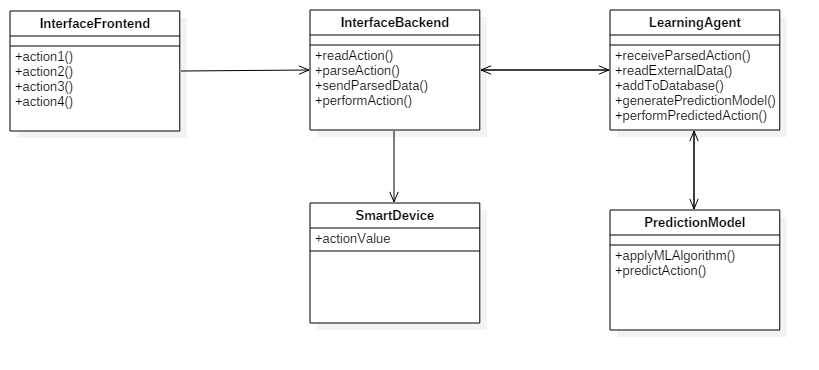
\includegraphics[width=\textwidth]{./Chapter5/ClassDiagram}
		\caption{Class Diagram}
	\end{figure}
	
	\paragraph{}
	This abstracts the major entities within our system as classes and shows the features they offer and the relationship between them.

	\subsection{Activity Diagram}
	\begin{figure}[H]
	\centering
	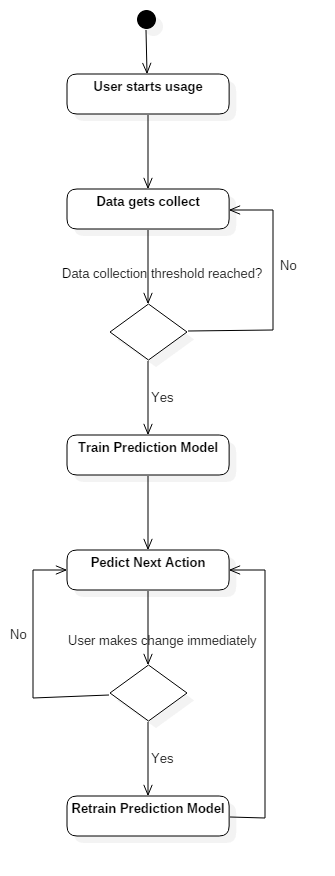
\includegraphics[scale=0.5]{./Chapter5/ActivityDiagram}
		\caption{Activity Diagram}
	\end{figure}
	\paragraph{}
	The activity diagram shows the flow of control through the process of our system. This system is designed to be non-terminating, so there is no halt in the flow. The system improves itself continually by realizing incorrect predictions.
	
	\subsection{Sequence Diagram}
	\begin{figure}[H]
	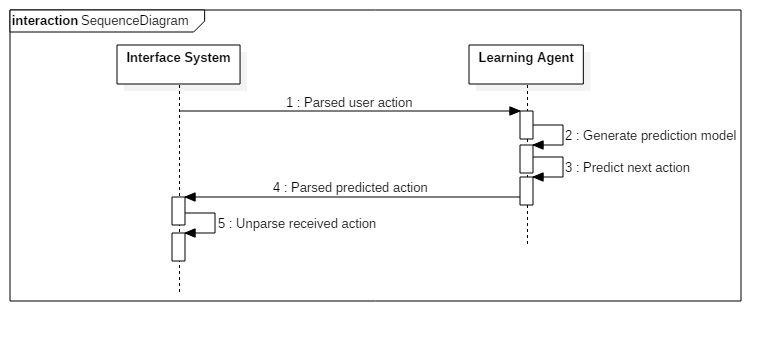
\includegraphics[width=\textwidth]{./Chapter5/SequenceDiagram}
		\caption{Sequence Diagram}
	\end{figure}
	\paragraph{}
	It shows the flow of objective-critical data and signals between some major entities within the system.


\begin{comment}
\begin{figure}
	\includegraphics[width=\textwidth]{Flower}
		\caption{A Flower}
\end{figure}
\end{comment}
	% System Architecture
	% UML Diagrams
		% Use Case Diagram
		% Class Diagram
		% Activity Diagram
		% Sequence Diagram
\chapter{Coding}

% Algorithm
% References to Technology
% Advantages
% Applications

\section{Algorithm}
<Stick LogReg history here.>

\section{References to Technology}

%Need to drop or reuse parts between "%%%...".
\begin{comment}
%%%%%%%%%%%%%%%%%%%%%%%%%%%%%%%%%%%%%%%%%%%%%%%%%%%%%%%%%%%%%%%%%%%%
\paragraph{Machine Learning}
Machine learning is a subfield of computer science that evolved from the study of pattern recognition and computational learning theory in artificial intelligence.In 1959, Arthur Samuel defined machine learning as a 
\begin{quote}
"Field of study that gives computers the ability to learn without being explicitly programmed".
\end{quote} Machine learning explores the study and construction of algorithms that can learn from and make predictions on data. Such algorithms operate by building a model from example inputs in order to make data-driven predictions or decisions, rather than following strictly static program instructions.
%%%%%%%%%%%%%%%%%%%%%%%%%%%%%%%%%%%%%%%%%%%%%%%%%%%%%%%%%%%%%%%%%%%%
\end{comment}

%Extra data. Doesn't seem relevant. It's the best page filler.
\begin{comment}
\subsubsection{Reinforcement Learning}
\paragraph{}
Reinforcement learning is an area of machine learning inspired by behaviorist psychology, concerned with how software agents ought to take actions in an environment so as to maximize some notion of cumulative reward.
\paragraph{}
Reinforcement learning differs from standard supervised learning in that correct input/output pairs are never presented, nor sub-optimal actions explicitly corrected. Further, there is a focus on on-line performance, which involves finding a balance between exploration (of uncharted territory) and exploitation (of current knowledge).

\paragraph{Temporal Difference Learning}
Temporal difference (TD) learning is a prediction-based machine learning method. It has primarily been used for the reinforcement learning problem. It learns by sampling the environment according to some policy, and is related to dynamic programming techniques as it approximates its current estimate based on previously learned estimates.
\paragraph{}
As a prediction method, TD learning considers that subsequent predictions are often correlated in some sense. In standard supervised predictive learning, one learns only from actually observed values: A prediction is made, and when the observation is available, the prediction is adjusted to better match the observation. The core idea of TD learning is that one adjusts predictions to match other, more accurate, predictions about the future.
\end{comment}

\begin{comment}
%%%%%%%%%%%%%%%%%%%%%%%%%%%%%%%%%%%%%%%%%%%%%%%%%%%%%%%%%%%%%%%%%%%%
\paragraph{Raspberry Pi}
The Raspberry Pi is an ARM-based Single Board Computer. It was initially launched in the UK to teach programming to school children but being very cheap yet powerful, it became a favorite among computer hobbyists around the world. The latest revision available at the time of writing this report is revision 3. Raspberry Pi runs it's own flavor of Linux based on Debian called Raspbian OS.

\paragraph{SciKit Learn}
SciKit Learn is an open-source machine learning library native to Python that is based on scipy and numpy. SciKit Learn implements a variety of machine learning algorithms in a very efficient way. It also comes with interfaces for many other popular languages.
%%%%%%%%%%%%%%%%%%%%%%%%%%%%%%%%%%%%%%%%%%%%%%%%%%%%%%%%%%%%%%%%%%%%
\end{comment}

\subsection{Raspberry Pi}
\paragraph{}
The Raspberry Pi is an ARM-based Single Board Computer. It was initially launched in the UK to teach programming to school children but being very cheap yet powerful, it became a favorite among computer hobbyists around the world. The latest revision available at the time of writing this report is revision 3. Raspberry Pi runs it's own flavor of Linux based on Debian called Raspbian OS.
\paragraph{}
This system is entirely designed using Python (for the back-end on Tier I and II) and HTML/Javascript (for the front-end on Tier I). Tier I is implemented on a Raspberry Pi 2, model B+ - an ARM Cortex A7-based 32-bit quad-core Single Board Computer with 512 MB RAM and frequency of 900 MHz, and running the default Raspbian OS. Python is installed by default on these systems. With this, we need to install the python-flask package - a lightweight framework for implementing robust WSGI applications.
\subsection{Python}
\paragraph{}
Python is an interpreted language with object oriented features.<Add python history and specs here>
\subsection{Flask (Python Library)}
\paragraph{}
<Add flask history here>
\subsection{SciKit Learn (Python Library)}
\paragraph{}
<Add SciKit Learn history here.>
\subsection{HTML}
\paragraph{}
<Add description.>
\subsection{JavaScript}
\paragraph{}
<Add history and description>
\subsection{REST Web APIs}
\paragraph{}
<Add description.>

\section{Advantages}

\begin{enumerate}

\begin{comment}
%%%%%%%%%%%%%%%%%%%%%%%%%%%%%%%%%%%%%%%%%%%%%%%%%%%%%%%%%%%%%%%%%%%%
\item \textbf{Machine Learning}
It is central to the functioning of any system that is based on learning complex models that often change dynamically, thus rendering hard coding of such models difficult if not impossible. Machine learning overcomes this hurdle by analyzing the model and trying to detect any patterns in it. Any changes in the pattern can also be detected by the system and the system can respond to it suitably.
%%%%%%%%%%%%%%%%%%%%%%%%%%%%%%%%%%%%%%%%%%%%%%%%%%%%%%%%%%%%%%%%%%%%
\end{comment}

\item \textbf{Raspberry Pi}
It's a cheap and yet complete, Linux-powered computer that can be used in lieu of many things like conventional microcontrollers, data sinks, and under-utilized workstations to name a few. It's size and cost also make it suitable to be used as a device interface in our project. Having a Python library to control its GPIO pins also makes it easier to program.

\item \textbf{Python}
<Add advantage>

\item \textbf{Flask}
<Add advantage over other WSGI frameworks>

\item \textbf{SciKit Learn}
By using this library, we are spared the effort of rewriting machine learning algorithms that we intend to use. Being in Python, importing and using this library becomes as easy as writing conventional Python code.

\item \textbf{JavaScript}
<Add advantage over other scripting languages>

\item \textbf{REST Web APIs}
<Add advantage over SOAP>
\end{enumerate}

\section{Applications}

\begin{enumerate}
\item \textbf{Machine Learning}
Being a broad field of study, it finds application in a wide variety of fields. One such new field is enhancing classical automation systems for smart homes and non-critical industrial operations by working on behavioral data in real-time. Although we are more focused on home automation, this system can be modified to suit even industrial systems.

\item \textbf{Raspberry Pi}
It is a complete computer system in itself and can be used in a variety of places. It's major applications include use as PC, smart device, hobby computer, teaching aid, IoT Hub etc.

\item \textbf{SciKit Learn}
Applications of this library are just as vast as that of machine learning itself. It has been used by various projects dealing with everything from artificial intelligence to big data analytics.
\end{enumerate}

	% Algorithm [TO BE ADDED]
	% Technology details used in the project
	% References to Technology
	% Advantages
	% Applications
\chapter{Result Sets}
<MORE INFO NEEDED> %previously, system-implementation-plan.tex

%\chapter{Work Done}

\section{<Section title>}

\subsection{<Sub-section title>}

\subsection{<Sub-section title>}
some text\cite{citation-2-name-here}, some more text
\subsection{<Sub-section title>}

\subsection{<Sub-section title>}

Refer figure \ref{fig:label}.

\begin{figure}[htb]
\centering

\includegraphics[scale=0.3]{./glider} % e.g. insert ./image for image.png in the working directory, adjust scale as necessary
\caption{<Caption here>}
\label{fig:label} % insert suitable label, this is used to refer to a fig from within the text as shown above
\end{figure}

\subsection{<Sub-section title>}


\section{<Section title>}

 %Currently not relevant.
%\chapter{Future Work}

<Future work here>
 % Currently not relevant.

\chapter{Testing}

% Test Plan: A document describing the scope, approach, resources and schedule of intended test activities. It identifies amongst others test items, the features to be tested, the testing tasks, who will do each task, degree of tester independence, the test environment, the test design techniques and entry and exit criteria to be used, and the rationale for their choice,and any risks requiring contingency planning. It is a record of the test planning process.
% Test Cases
% Test Results

\section{Test Plan}
\paragraph{}
This is a document describing the testing scope and activities. It is the basis for formally testing components of this software project.

\subsection{Scope}
%<What all is going to be tested>
\paragraph{}
Testing will be performed only on functional components of the system. These include the two main modules corresponding to Tier I and Tier II. Besides this, we don't yet have a plan to perform any other non-functional tests. This testing strategy suffices, as the project itself is not very vast. Listing more formally, the components to be tested are:
\begin{enumerate}
\item Module I (Tier I)
	\begin{enumerate}
	\item Web API for device control.
	\item Individual functions involved in maintaining device state changes and reporting them to Module II.
	\end{enumerate}
\item Module II (Tier II)
	\begin{enumerate}
	\item Web API for Learning Service.
	\item Individual functions involved in data accumulation and learning process.
	\end{enumerate}
\end{enumerate}

\subsection{Not in Scope}
%<What all is NOT going to be tested - how the client views the WebUI, conformance of inter-tier interfaces to standards>
%<Why - not very relevant to the core idea being demonstrated, unnecessary for this demonstration>
\paragraph{}
We won't be performing any tests to verify if the users interfaces are satisfactory and convenient for the user. This doesn't form a core part of the idea that we are trying to demonstrate through this project.
\paragraph{}
This test plan also doesn't include any tests for verifying conformance of the implemented APIs to any particularly defined interface standards. Again, this hinders the simplicity of demonstration of the intended idea - involving a combined application of SaaS, IoT, and ML to solve the problem of home automation using predictive learning.
\paragraph{}
Below is a list of things that have been declared out of scope for this test, for the reasons stated above:
\begin{enumerate}
\item User Interface Testing.
\item Testing conformance of components (especially the web APIs) to set standards.
\end{enumerate}

\subsection{Assumptions}
%<All the conditions that need to hold true for us to be able to proceed successfully - client-tier I network always available>
\paragraph{}
We need to make certain assumptions regarding the environment we operate in, and the tests we cannot perform - for reasons that otherwise deem development, testing and operation impractical to achieve. This can be a long list if each minute detail is taken into account, so we need to limit it to the core hardware and software components that directly impact us. Some of these assumption are:
\begin{enumerate}
\item The network infrastructure connecting the Clients to Tier I will always be available.
\item The clients themselves will always have access to suitable devices that will be used to connect to the automation system.
\item Connection between the Tier I application and the Tier II service will be available most of the time. Occasional unavailability of Tier II service is tolerable.
\item There are no security threats that need to be addressed within the house-wide network that the client, Tier I and Tier II are all a part of.
\end{enumerate}

\subsection{Environment}
%<What kind of environment requirements exist. The software and hardware used for testing.>
\paragraph{}
Modules I and II will have to be tested independently. This will be done by performing pre-designed unittests. Each individual component (that is to say, each "function") will be tested by passing a value to it and checking if the returned value matches expected value. Module I will be hosted on the Raspberry Pi, that is the controller; while Module II will be hosted on the PC, and provide learning service to Module I.
\paragraph{}
Each test case is intended to be executed on the device that will host the component being tested. This will keep the test environment and usage environment consistent, leading to more robust tests. The developed tests will have to be run manually, as we don't plan on automating these tests.

\subsection{Tools}
%<Tools used to test the code. Python's unittest library, in this case.>
\paragraph{}
Due to the simplicity of this project, we will not be using any sophisticated test or result management software to keep track of tests. The entire test code will be developed using just one Python language tool - the unittest library. The unittest library is the default testing library that comes with the standard library itself. We will be using this to make sure the components behave the way we expect them to.

\subsection{Exit Criteria}
%<When to stop testing - when tests for all "units" are satisfied.>
\paragraph{}
The exit criteria for the test will be simple - success for all tests implies end of testing. Conformance of all components to the test criteria will be necessary to signal an exit from the tests.

\section{Test Cases}
%<Define cases for each "unit" that is within scope of testing>
\paragraph{}
Each module will have its own set of test cases for each of the components it contains.

\section{Test Results}
<Expected vs Actual>
	% Test Plan [TO BE ADDED]
	% Test Cases [TO BE ADDED]
	% Test Results [TO BE ADDED]
\chapter{Conclusion}

\paragraph{}
With the rise of Internet of Things and more powerful computers, we will be able to achieve Utopian homes using Smart Automation powered by Machine Learning Algorithms of higher complexity than Temporal Difference based Reinforcement Learning running on current data. More data will lead to better prediction of potential user action which will help us lead more comfortable lives. Physically challenged people can also benefit from such systems which will eventually make them more independent, as more and more data gets collected to predict such users' habits. The impact of this technology on human lives will be deep and possibly every human-machine interface in the future will have some form of machine learning powered intelligent assistance. Changes in user habits can also be used to predict a lot of other things about the user such as the user's physical and mental health. In fact, many current technologies aim to provide basic level medical assistance using machine learning systems.
\cleardoublepage
%\pagebreak
\phantomsection
%\stepcounter{\value{\thechapter}}
\addcontentsline{toc}{chapter}{\protect\numberline{10} References}
\begin{thebibliography}{99}

%\bibitem{citation-1-name-here}<Name of the reference here>,\ \url{<url here>}

\bibitem{}Panos Luridas, Christof Ebert,``Machine Learning", IEEE Computer Society, 2016

\bibitem{}Jeremie Saives, Clement Pianon, and Gregory Faraut, ``Activity Discovery and Detection of Behavioral Deviations", in IEEE TRANSACTIONS ON AUTOMATION SCIENCE AND ENGINEERING, 2016

\bibitem{}Christopher Osiegbu, Seifemichael B. Amsalu, Fatemeh Afghah, Daniel Limbrick and Abdollah Homaifar, ``Design and Implementation of an Autonomous Wireless Sensor-based Smart Home", IEEE, 2015

\bibitem{}Wesllen S. Lima, Eduardo Souto, Richard W. Pazzi, Ferry Pramudianto, ``User Activity Recognition for Energy Saving in Smart Home Environment", IEEE Symposium on Computers and Communication, 2015

\bibitem{}Vahid Ghasemi, Ali Akbar Pouyan, ``Activity Recognition in Smart Homes Using Absolute Temporal Information in Dynamic Graphical Models", IEEE Computer Society, 2015

\bibitem{}Beichen Chen, Zhong Fan, and Fengming Cao, ``Activity Recognition Based on Streaming Sensor Data for Assisted Living in Smart Homes", IEEE Computer Society, 2015

\bibitem{}K.S.Gayathri, Susan Elias, S.Shivashankar, ``Composite activity recognition in smart homes using Markov Logic Network", IEEE Computer Society, 2015

\bibitem{}Labiba Gillani Fahad \& Muttukrishnan Rajarajan,``Anomalies detection in  smart-home activities", in IEEE 14th International Conference on Machine Learning and Applications, 2015

\bibitem{}Z. Meng, and J. Lu, ``A Rule-based Service Customization Strategy Context- aware Automation for Smart Home", in IEEE TRANSACTIONS ON MOBILE COMPUTING, 2014

\bibitem{}Chiming Chang, Paul-Armand Verhaegen, Joost R. Duflou, ``A Comparison of Classifiers for Intelligent Machine Usage Prediction", IEEE Compuer Society, 2014

\bibitem{}Parisa Rashidi, Student Member, IEEE, and Diane J. Cook, Fellow, ``Keeping the Resident in the Loop: Adapting the Smart Home to the User", in IEEE TRANSACTIONS ON SYSTEMS, MAN, AND CYBERNETICS, 2009

\end{thebibliography}
\cleardoublepage
%\pagebreak
\phantomsection
\addcontentsline{toc}{chapter}{Plagiarism Check Report}
\chapter*{Plagiarism Check Report}
\cleardoublepage
%\pagebreak
\phantomsection
\addcontentsline{toc}{chapter}{Paper Published Details}
\chapter*{Paper Published Details}

\end{document}
